\chapter{Project Architecture and Design}

In the following text, the author will describe the architecture and design of the Thesis Management System including functional and non-functional requirements of the client.

\section{Functional requirements}

\begin{enumerate}
    \item User management\\
    The system allows to CRUD users. A user contains fields full name, email and password.

    \item Registration\\
    An anonymous user can sign up.

    \item Thesis topic management\\
    The system allows to create, read, update and delete (CRUD) a thesis topic. A topic contains fields title and description in two languages.

    \item Category management\\
    The system allows to CRUD categories. A category contains fields title and description.

    \item Thesis topic can be added to categories.\\
    Topics can be added to one or more categories which allows a user to browse topics in a category.

    \item Tags can be assigned to a thesis topic\\
    There can be zero or more tags assigned to a thesis topic.

    \item Thesis topic contains field for an external supervisor (owner)\\
    The supervisor has the authority to manage thesis topics created by them.

    \item University management\\
    The system allows to CRUD universities. A university contain a field for the name of the university.

    \item Thesis topic contains field for list of universities\\
    This field contains the list of universities that the topic is offered to. A thesis topic can be offered to one or more universities.

    \item Thesis topic contains field for list of supervisors\\
    This field contains the list of university supervisors, each supervisor is assigned a university that they supervise at. A thesis topic can have zero or more university supervisors.

    \item Thesis topic contains field for list of types\\
    This field contains the list of types (i.e. diploma, bachelor). A thesis topic can have zero or more types.

    \item Application management\\
    The system allows to CRUD applications.

    \item Students can apply for a thesis topic\\
    The applicant chooses the type and the university that they apply to.

    \item Application can be approved

    \item Thesis topic can be enabled or disabled

    \item Thesis topics can be filtered\\
    The system allows to filter thesis topics by university, type, owner or title.

    \item Thesis management\\
    The system allows to CRUD theses. A thesis contains fields title, description, thesis topic, assignee, supervisor, abstract, type and university.

    \item Tags can be assigned to a thesis\\
    There can be zero or more tags assigned to a topic.

    \item Thesis contains field status\\
    Status can be either `in progress', `finished', `failed' or `postponed'.

    \item Thesis contains field grade\\
    One of A, B, C, D, E or F.

    \item Theses can be filtered\\
    The system allows to filter theses by title, supervisor, assignee, status, grade, type or university.

    \item Theses and thesis topics can be filtered by tags\\
    The system allows to list theses or thesis topics that contains a particular tag.

    \item File management for theses\\
    The system allows to upload files to a thesis.

    \item Discussion for thesis topics and theses\\
    A logged in user can comment on thesis topics and theses.

    \item Private comments\\
    Comments that are not visible to students can be created.

    \item Full text search\\
    Theses and thesis topics can be searched by a full text search engine.

    \item Frequently Asked Questions (FAQ) management\\
    The system allows to CRUD Frequently Asked Questions. One frequently asked question contains fields question, answer and locale.

\end{enumerate}

\newpage

\subsection{Use case diagram}

\begin{figure}[H]
    \centering
        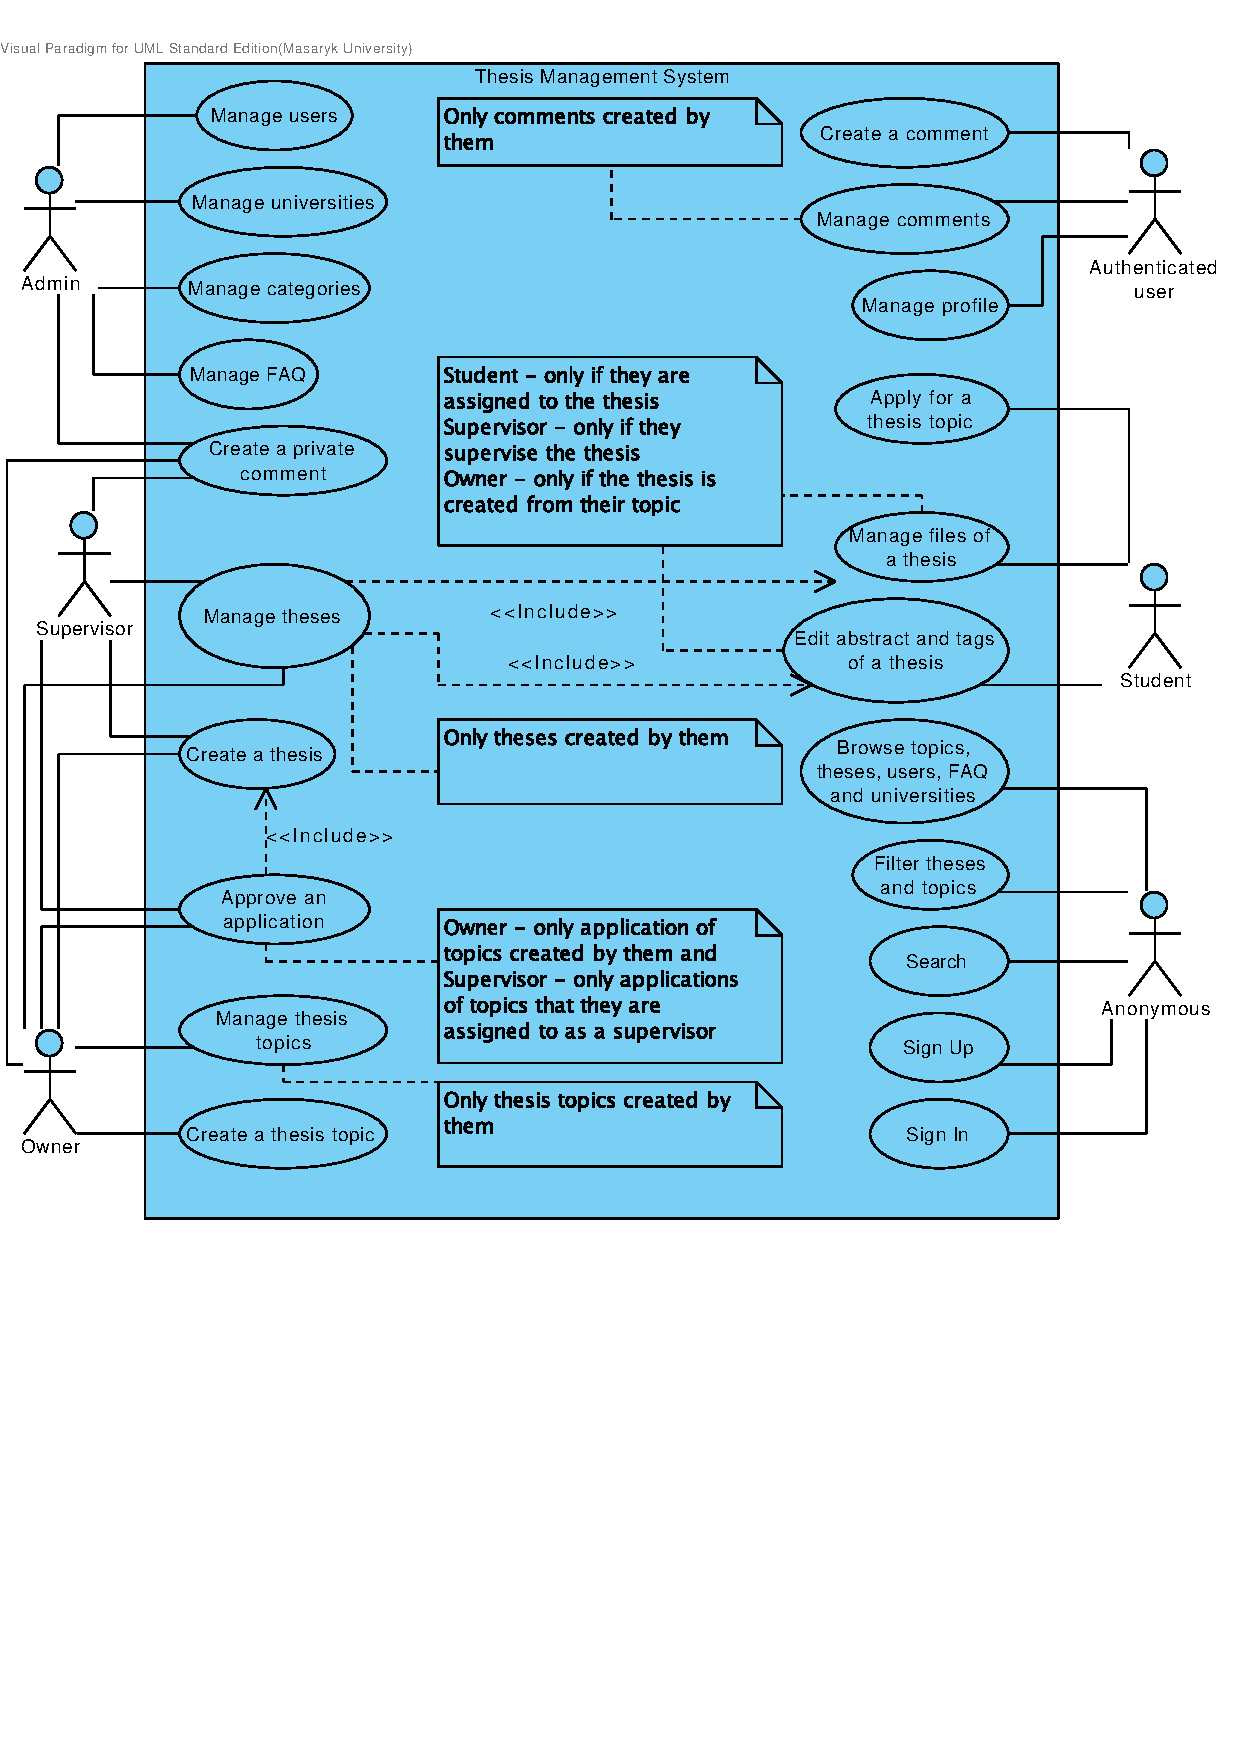
\includegraphics[trim=0 250 10 30, clip, keepaspectratio, width=\textwidth]{./images/use-case.pdf}
    \caption{Use case diagram of the Thesis Management System}
\end{figure}

\section{Non-functional requirements}

\begin{enumerate}
    \item Grails platform\\
    The system is implemented using platform Grails.

    \item Authentication and authorization\\
    The system is secured and there are four roles -- \textbf{Administrator} that can manage users, categories, FAQ and universities, \textbf{Owner} that can create thesis topics and manage thesis topics created by them, \textbf{Supervisor} that can create theses and manage theses created by them and \textbf{Student} that can apply for a thesis topic.

    \item Performance\\
    The system offers reasonable performance at least up to five hundred created thesis topics, theses, users and universities.

    \item Deployment\\
    The system is deployed on OpenShift using any cartridge other than Do It Yourself.

    \item License\\
    The system is licensed under any GPL compatible license.

    \item Backup\\
    Create a shell script for backing up the database.

    \item Internationalization and localization\\
    The system is internationalized and localized in English and Czech.

\end{enumerate}

\section{Domain model}

\faketext[30]